\aufgabe{}{

In exercise 2 on sheet 1 you received a dataset with 11 observations and two features:

\begin{table}[ht]
\centering
\begin{tabular}{rrrrrrrrrrrr|r}
\hline
& 1 & 2 & 3 & 4 & 5 & 6 & 7 & 8 & 9 & 10 & 11 & $\sum_{i = 1}^n$ \\ 
\hline
y & -7.90 & -6.08 & -3.74 & -1.18 & -1.23 & -0.55 & 0.05 & 0.88 & 4.74 & 2.93 & 2.55 & -9.53\\ 
x1 & -1.00 & -0.80 & -0.60 & -0.40 & -0.20 & 0.00 & 0.20 & 0.40 & 0.60 & 0.80 & 1.00 & 0 \\ 
x2 & 0.95 & 0.65 & 0.40 & 0.07 & 0.06 & 0.02 & 0.02 & 0.14 & 0.34 & 0.60 & 0.98 & 4.23 \\ 
\hline
\end{tabular}
\end{table}

The last column corresponds to the sum of values of each row.\\

Instead of 11 data points you now received a dataset with 1000 data points from 
the same data generating process as above. 
You fitted a linear model to the data 
$\fh(\xv) = \hat \beta_0 + \hat\beta_1 \xv_1 + \hat\beta_2 \xv_2 + \hat\beta_3 \xv_1 \xv_2$
The following plots show the PDP (first row) and ALE (second row) for $x_1$ and $x_2$. 
\begin{enumerate}
\item Interprete the plots with respect to the feature effect of $x_1$ and $x_2$. 
\item Would you rather trust the PDP or ALE plot? Give reasons for your 
decision. 


\begin{center}
  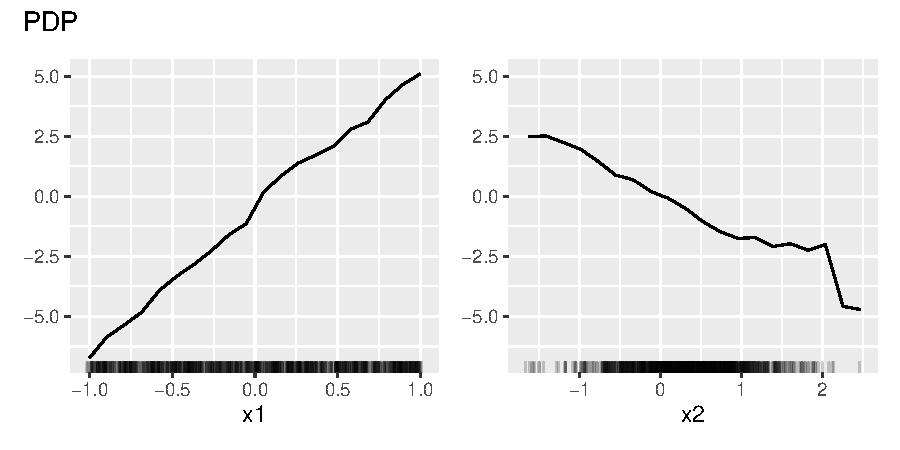
\includegraphics[width=\maxwidth]{figure/PDP_Plot.pdf}
\end{center}


\begin{center}
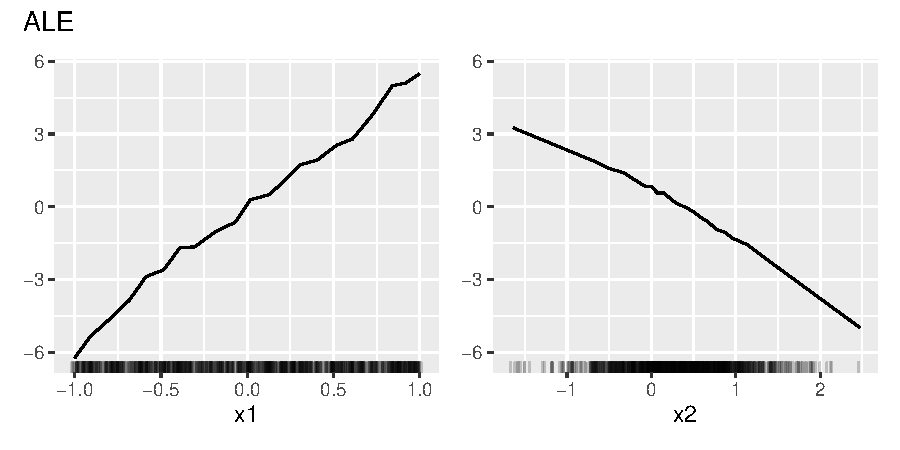
\includegraphics[width=\maxwidth]{figure/ALE_Plot.pdf}
\end{center}

\end{enumerate}
}
